% !TeX root = ../../book.tex
\section{学而时习之}\label{sec:section1.5}

我们以一些练习来结束本章,这些练习结合了我们前面讨论的一些思想,给你一个机会来实践你之前所学,抑或只是为了让你保持头脑清醒。尽可能多地尝试,并与朋友们讨论可能的解决方案,看看他们的想法。不过,归根结底,只需将其视为保持大脑灵活的一种方式!

\begin{exercise}
    一只苍蝇停在一辆以每小时 $60$ 公里的速度向前疾驰的火车前面。在同一条轨道上,前方 $300$ 公里处,另一列火车正以每小时 $60$ 公里的速度向前一列火车疾驰而来。此时,当火车相距 $300$ 公里时,苍蝇以每小时 $90$ 公里的速度起飞,不断地在火车之间的轨道上方来回飞行,到达火车时瞬间转身。在两列火车相撞,挤压到它们之间苍蝇之时,苍蝇总共飞了多少距离?你是怎么想出来的?尝试将情况泛化到一列火车以 $a$ km/hr 行驶,另一列以 $b$ km/hr 行驶,而苍蝇以 $c$ km/hr 飞行。
\end{exercise}

\begin{exercise}
    政府铸币厂受委托铸造一批金币。铸币厂有 $20$ 台机器,每台机器生产重 $5$ 克的硬币。一天,铸币厂的工头发现有些硬币轻了,他对机器进行了盘查,发现其中一台机器铸造出的硬币为 $4$ 克,而其他 $19$ 台机器工作正常。他决定化不利为有利,以此找到最聪明的员工,接下来提拔他。他告诉工人,只有一台机器正在生产 $4$ 克的硬币,他们需要确定哪台机器坏了。作为员工,你可以在秤上称一次,但\emph{只能}称一次。你可以放置任意选定机器生产的任意数量的硬币,但必须将它们放置在一起,并且只会看到所有硬币的总重量,以克为单位。你要如何做,才能准确地确定哪台机器坏了?
\end{exercise}

\begin{exercise}
    在国际象棋中,皇后可以垂直、水平或沿对角线任意方向移动任意数量的格子。尝试在一个标准的 $8 \times 8$ 棋盘上放置 $8$ 个皇后,使得任意皇后都不会攻击到其他皇后(也就是说,\emph{没有}皇后可以下一步立即吃掉另一个皇后)。展示一种方法来做到这一点或证明这是不可能的。如果你找到了一种方法,你认为有多少种不同的方法可以做到这一点?如果你证明这是不可能的,请找出最多多少个皇后可以满足条件。以这种方式,你最多可以在棋盘上放置多少个皇后?
\end{exercise}

\begin{exercise}
    在一个标准的 $8 \times 8$ 棋盘上,在对角处移除 $2$ 个格子,比如右上角和左下角。你能用 $2 \times 1$ 的多米诺骨牌覆盖所有剩余的方格,且所有的多米诺骨牌都不\emph{重叠}吗?(注意:这被称为棋盘\emph{密铺}。)为什么能或为什么不能?在一般情况下,如果有一个 $n \times n$ 棋盘呢?你的答案取决于 $n$ 吗?为什么会这样呢?
\end{exercise}

\begin{exercise}
    考虑一个标准的 $8 \times 8$ 棋盘,对角上移除两个相邻的方块。(如图。)你能用 T 形四联骨牌密铺这个棋盘吗?(如图。)如果可以,怎么做到?如果不能,为什么不能?

    \begin{center}
        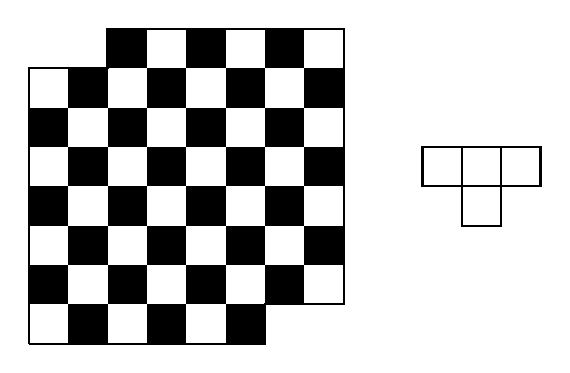
\begin{tikzpicture}[thick, scale=0.5, x=1cm]
            \foreach \x in {0,...,5}
                {
                    \pgfmathparse{mod(\x,2) ? "black" : "white"}
                    \edef\colour{\pgfmathresult}
                    \path[fill=\colour] (\x, 0) rectangle ++ (1,1);
                }
            \foreach \x in {0,...,7} 
                \foreach \y in {1,...,6}
                    {
                        \pgfmathparse{mod(\x+\y,2) ? "black" : "white"}
                        \edef\colour{\pgfmathresult}
                        \path[fill=\colour] (\x,\y) rectangle ++ (1,1);
                    }
            \foreach \x in {2,...,7}
                {
                    \pgfmathparse{mod(\x+1,2) ? "black" : "white"}
                    \edef\colour{\pgfmathresult}
                    \path[fill=\colour] (\x, 7) rectangle ++ (1,1);
                }
            \draw (0,0)--(6,0)--(6,1)--(8,1)--(8,8)--(2,8)--(2,7)--(0,7)--(0,0);
            \draw (10,4) rectangle ++ (1,1);
            \draw (11,4) rectangle ++ (1,1);
            \draw (12,4) rectangle ++ (1,1);
            \draw (11,3) rectangle ++ (1,1);
        \end{tikzpicture}
    \end{center}

    一般情况下,如果是 $n \times n$ 棋盘呢?你的答案取决于 $n$ 吗?为什么会这样呢?
\end{exercise}

\begin{exercise}
    给定一个实数 $x$,我们令 $\lfloor x \rfloor$ 表示小于(或等于)$x$ 的最大整数,让 $\lceil x \rceil$ 表示大于(或等于)$x$ 的最小整数。例如,$\lfloor 6.02 \rfloor = 6$, $\lfloor 6.99999 \rfloor = 6$, $\lfloor 6 \rfloor = 6$, $\lfloor -6.5 \rfloor = -7$ 。

    尽可能为以下表达式的值确定更具体和简洁的表示形式。(你可能需要找到一些不同的表达式,具体取决于 $x$。)

    \begin{enumerate}
        \item $\lfloor x \rfloor + \lfloor 1-x \rfloor$ 
        \item $\lceil x \rceil + \lceil 1-x \rceil$
        \item $\lfloor x \rfloor + \lceil x \rceil$
        \item $\frac{\lfloor x \rfloor}{x}$
        \item $\lfloor x^2 \rfloor - \lfloor x \rfloor ^2$
        \item $\lceil x^2 \rceil - \lceil x \rceil^2$
    \end{enumerate}
\end{exercise}

\begin{exercise}
    求三个自然数 $a,b,c$,使得没有子集的和能被 $3$ 整除。即求 $a,b,c$,使得下列和都不能被 $3$ 整除:$a,b,c,a + b,a + c,b + c,a + b + c$。这可能吗?为什么能或为什么不能?

    尝试用 $4$ 个数做同样的事情:求自然数 $a,b,c,d$,使得没有子集的和能被 $4$ 整除。这可能吗?为什么能或为什么不能?

    尝试泛化一下,你能说一说找到 $n$ 个自然数使得所有子集的和都不能被 $n$ 整除吗?
\end{exercise}

\begin{exercise}
    回想一下我们通过点和彩色线条解决朋友趋势问题的方法。对于这个问题,我们想解决类似的情况,我们有一定数量的点,需要绘制所有可能的线,让任意两点都恰好由一条线连接,但在这种情况下,我们不关心颜色,所以我们可以说所有的线都是黑色的。你能用 $3$ 个点画出这个图形,使所有的线都不交叉吗?$4$ 个点呢?$5$ 个?$6$ 个?为什么行或者为什么不行?试着解释为什么这些图形中的任何一个都不可能实现。如果你不能实现 $0$ 次交叉,你可能达到的最小数量是多少?
\end{exercise}

\begin{exercise}
    画一个圆圈。沿圆周放置 $3$ 个点。我们想给点之间的部分着色(每个部分只有一种颜色),两个相同颜色不相邻。我们需要多少种颜色?如果我们在圆周上放置 $4$ 个点呢?$5$ 个呢?尝试泛化到 $n$ 个点。你能说一下所需的颜色数量吗?
\end{exercise}

\begin{exercise}
    假设你有一个装满袜子的抽屉。里面有 $2$ 双蓝色袜子、$3$ 双红色袜子和 $4$ 双绿色袜子。(同时假设左袜子和右袜子是无法区分的。)一天早上,你很着急,开始随机抓袜子,一次抓一只,将所有袜子拿在手上,直到你有一双为止。你需要从抽屉里拿出多少只袜子才能\emph{保证}你手上有一双袜子?

    如果每种颜色的袜子是以前的两倍,您的答案会有什么变化?如果我们每种颜色有 $3$ 双袜子,颜色分别是红色、绿色、蓝色、黄色和棕色,会怎样?如果我们每种颜色有 $n$ 双袜子,共有 $m$ 种颜色,又会怎样?
\end{exercise}

\begin{exercise}
    深夜,一行四人在回家路上来到了桥头。这座桥又旧又晃,一起过去不安全。他们只有一个手电筒,光线的强度只能同时为两个人照亮道路。每个人对这座桥的舒适程度不同,所以他们会以不同的速度过桥。一人过桥需要 $5$ 分钟,一人需要 $10$ 分钟,一人需要 $15$ 分钟,一人需要 $20$ 分钟。如果两个人一起过桥,就按照较慢的人的步调通过。四人全部过桥需要多长时间?你能找到给出绝对最短时间的方法吗?
\end{exercise}

\begin{exercise}
    考虑美元硬币的常见面额:$1$ 美分、$5$ 美分、$10$ 美分和 $25$ 美分。你需要在口袋里随身携带什么硬币才能\emph{保证}你可以准确地支付 $0$ 美分到 $100$ 美分之间的任何价格?是否有几组可能的硬币可以实现这一目标?具有此属性的硬币的最小总价值是多少?是否有几组可能的硬币具有相同的最小总值?
\end{exercise}

\begin{exercise}
    设 $a,b,c$ 为实数,其中 $a \ne 0$。以下``伪证明'' $-\frac{b}{2a}$ 是方程 $ax^2 + bx + c = 0$ 的解(如果有的话)有什么问题?

    \textbf{``伪证明'':}设 $x$ 和 $y$ 为方程的解。从 $ax^2+bx+c = 0$ 中减去 $ay^2+by+c = 0$ 得 $a(x+y)(x-y)+b(x-y) = 0$。因此,$a(x+y)+b = 0$,所以 $x + y = -ba$。因为 $x$ 和 $y$ 是\emph{任意}解,我们可以用 $x = y$ 重复这个计算。因此,$2x = -ba$,因此 $x = -2ba$ 是一个解。``$\square$''
\end{exercise}

\begin{exercise}
    解释为什么 $(-1)(-1) = 1$。假设你正在为一位对此事实持怀疑态度并需要被说服的具有相同智力水平的同学撰写证明。仅仅说``因为它就是这样!''是\emph{不够的}。试着想出一个有用的\emph{几何}或\emph{物理}解释,某种令人难忘的论证。
\end{exercise}

\begin{exercise}
    对于以下方程,确定满足它们的所有实数:

    \begin{enumerate}
        \item $\vert x-2 \vert = \vert x-3\vert$
        \item $\vert 2x-1 \vert = \vert 2x-3\vert$
        \item $\vert 2x-2 \vert = \vert 2x-3\vert$
        \item $\vert x+1 \vert = \vert x-5\vert$
        \item $\vert x-1 \vert + \vert x-2 \vert = \vert x-3\vert$
    \end{enumerate}
\end{exercise}

\begin{exercise}
    \textbf{逻辑俱乐部第一规则...:}要加入逻辑俱乐部,必须决定\emph{始终}说真话或\emph{始终}说谎话。逻辑俱乐部的成员知道谁说谎,谁诚实。我不是逻辑俱乐部的成员,但我在街上遇到三名成员发表以下言论:

    \begin{itemize}
        \item 杰克:``我们三个都是骗子。''
        \item 泰勒:``我们三人中只有两人是骗子。'' 
        \item 查克:``杰克和泰勒是骗子。''
    \end{itemize}

    如果可以的话,我应该相信谁?
\end{exercise}

\begin{exercise}
    求解满足方程 $\sqrt{x - 1} = x - 3$ 的所有实数解。解释你的工作,并尝试说明为什么你的答案是\emph{唯一}答案。
\end{exercise}

\begin{exercise}
    你有两根保险丝。每个都会燃烧整整一个小时。但是,保险丝不一定相同,并且不会以恒定速率燃烧。你身上只有一个打火机和这两根保险丝。你能精确测量 $45$ 分钟吗?如果能,请解释如何实现。如果不能,请解释原因。
\end{exercise}

\begin{exercise}
    这个问题是原题的变体,其原型最早出现在 1926 年的《星期六晚邮报》上!

    三个朋友凑钱买了一大袋 \text{M\&M} 糖果。他们把盒子带回了他们的公寓,并决定第二天在聚会上分享这袋糖果。

    夜里,第一个人醒来,想吃点零食。他决定现在就吃掉他那份糖果,第二天不吃了。他打开袋子,将 \text{M\&M} 糖果分成三等份,但发现还剩下一粒。他认为多吃一个不会有什么坏处,于是就吃掉了自己那份糖果外加多出来的那粒糖果,然后把剩下的糖果放回袋子里。

    过了一会儿,第二个人做了同样的事情。他醒来觉得肚子饿了,把袋子里剩下的糖果分成三份,吃掉了自己那份外加多出来的那粒糖果。

    又过了一会儿,第三个人也做了同样的事情,吃掉了自己那份外加多出来的那粒糖果。

    第二天聚会上,他们把剩下的糖果分成三等份并享用了。(当然,没人承认他们所做的一切)。

    一开始袋子里有多少颗 \text{M\&M} 糖果?最小可能的数字是多少?
\end{exercise}

\begin{exercise}
    给定一个实数列表,它们的\emph{算术}平均数定义为它们的总和除以项数,它们的\emph{几何}平均数定义为它们的乘积开项数次方根。也就是说,假设 $x_1, x_2, \dots , x_n$ 为实数,则算术平均数为
    \[\frac{x_1+x_2+ \dots + x_n}{n}\]
    几何平均数为
    \[\sqrt[n]{x_1 \cdot x_2 \cdot \dots \cdot x_n}\]
    (注意:一个数的 $n$ 次方根等于该数的 $\frac{1}{n}$ 次方。)

    你能找到两个数,其算术平均数和几何平均数\emph{相等}吗?你能找到两个数,其算术平均数严格大于几何平均数吗?反过来呢?

    用三个数字、四个数字等等重复此操作。您能从中识别出一般模式吗?
\end{exercise}

\begin{exercise}
    考虑不定方程 $6x+ 15y = 93$。我们想找到一些\emph{积分}解;也就是说,我们想找到满足方程的 $x$ 和 $y$ 的\emph{整数}(自然数、零和负自然数)解。

    \begin{enumerate}
        \item 找到一个解,其中 $x$ 和 $y$ 都是正整数。用几句话描述你是如何找到这个解的。
        \item 找到一个解,其中 $x$ 或 $y$ 一个值为正,另一个为负。再次说明你是如何找到个解的。
        \item 你认为有多少组解?尝试写下所有可能解的特征,或描述你是如何找到所有这些解的。
    \end{enumerate}
\end{exercise}

\begin{exercise}
    \textbf{幻方}是一个 $n \times n$ 数组,它包含从 $1$ 到 $n^2$ 的每个数字,并且具有每行和每列(以及两条主对角线)数字和为相同数字的属性。

    例如,下面是一个 $3 \times 3$ 幻方:

    \begin{center}
        \begin{squarecells}{3}
            8 & 1 & 6 \nl
            3 & 5 & 7 \nl
            4 & 9 & 2 \nl
        \end{squarecells}
    \end{center}

    请注意,在这种情况下,每行/列/对角线的所谓\textbf{幻数和}为 15。

    你能找到一个 $n \times n$ 幻方的幻数和公式吗?

    (提示:我们在本章中发现过一个有用的结论。)
\end{exercise}

\begin{exercise}
    小于或等于 $1000$ 的整数中有多少整数至少有一位为 $1$?例如 $1$、$12$ 和 $511$。
\end{exercise}

\begin{exercise}
    我们有若干堆考拉熊。为了打散它们,我们从每堆中取出一只考拉熊,然后将所有这些考拉熊放入新的一堆中。例如,如果我们从大小为 $1$、$4$ 和 $4$ 的考拉熊堆开始,那么我们将以大小为 $3$、$3$ 和 $3$ 的考拉熊堆结束;或者,如果我们从大小为 $3$ 和 $4$ 的考拉熊堆开始,我们将以大小为 $2$、$2$ 和 $3$ 的考拉熊堆结束。

    我们\textbf{有}可能\emph{只执行一次}此操作并最终得到与开始时\emph{完全相同的堆大小}(它们的顺序无关紧要;只有\emph{大小}重要)。

    确定所有具有此性质的堆的集合,并解释为什么它们是唯一的。

    \emph{提示}:具有此性质的初始情况示例是当我们只有一堆大小为 $1$ 的堆时。我们执行该操作会再次获得一堆大小为 $1$ 的堆。搞定。

    \emph{提示 2}:一定要解释为什么你的情况是\emph{唯一}有效的。我们如何确定你没有遗漏某些答案呢?
\end{exercise}